\documentclass[12pt]{article}
\usepackage{graphicx} % Required for inserting images
\usepackage{mathtools}
\usepackage{amsmath}
\usepackage{gvv-book}
\usepackage{gvv}
\usepackage[shortlabels]{enumitem}
\usepackage{multicol}

\title{\textbf{9.4.16}}
\author{\textbf{EE25BTECH11004 - Aditya Appana}}
\date{October 4, 2025}
\renewcommand{\labelenumi}{\Alph{enumi})}
\begin{document}

\maketitle

\section*{Question}
Find the roots of the following quadratic equation graphically:
$$2x^2-7x+3=0$$
\section*{Solution}

The parabola can be represented in vector form as:
\begin{align}
    \vec{x^T}\myvec{1&0\\0&0}\vec{x} - \myvec{\frac{7}{2} \\ \frac{1}{2}}^T\vec{x} + \frac{3}{2} = 0
\end{align}\\
The y-axis can be represented in vector form as:
\begin{align}
    \vec{x} = \kappa\myvec{1\\0}
\end{align}\\
We need to find the intersection of this line with the parabola, which can be done by substituting equation (2) in (1):
\begin{align}
    \kappa\myvec{1\\0}^T\myvec{1&0\\0&0}\kappa\myvec{1\\0} - \myvec{\frac{7}{2} \\ \frac{1}{2}}^T\kappa\myvec{1\\0} + \frac{3}{2} = 0\\
    2\kappa^2-7\kappa+3=0\\
    (2\kappa - 1)(\kappa -  3) = 0\\
    \kappa = \frac{1}{2}, 3
\end{align}\\
Therefore, the points of intersection \textit{i.e.} the \textbf{roots} are $\myvec{\frac{1}{2}\\0}$ and $  \myvec{3\\0}$.

\begin{figure}[H]
    \centering
    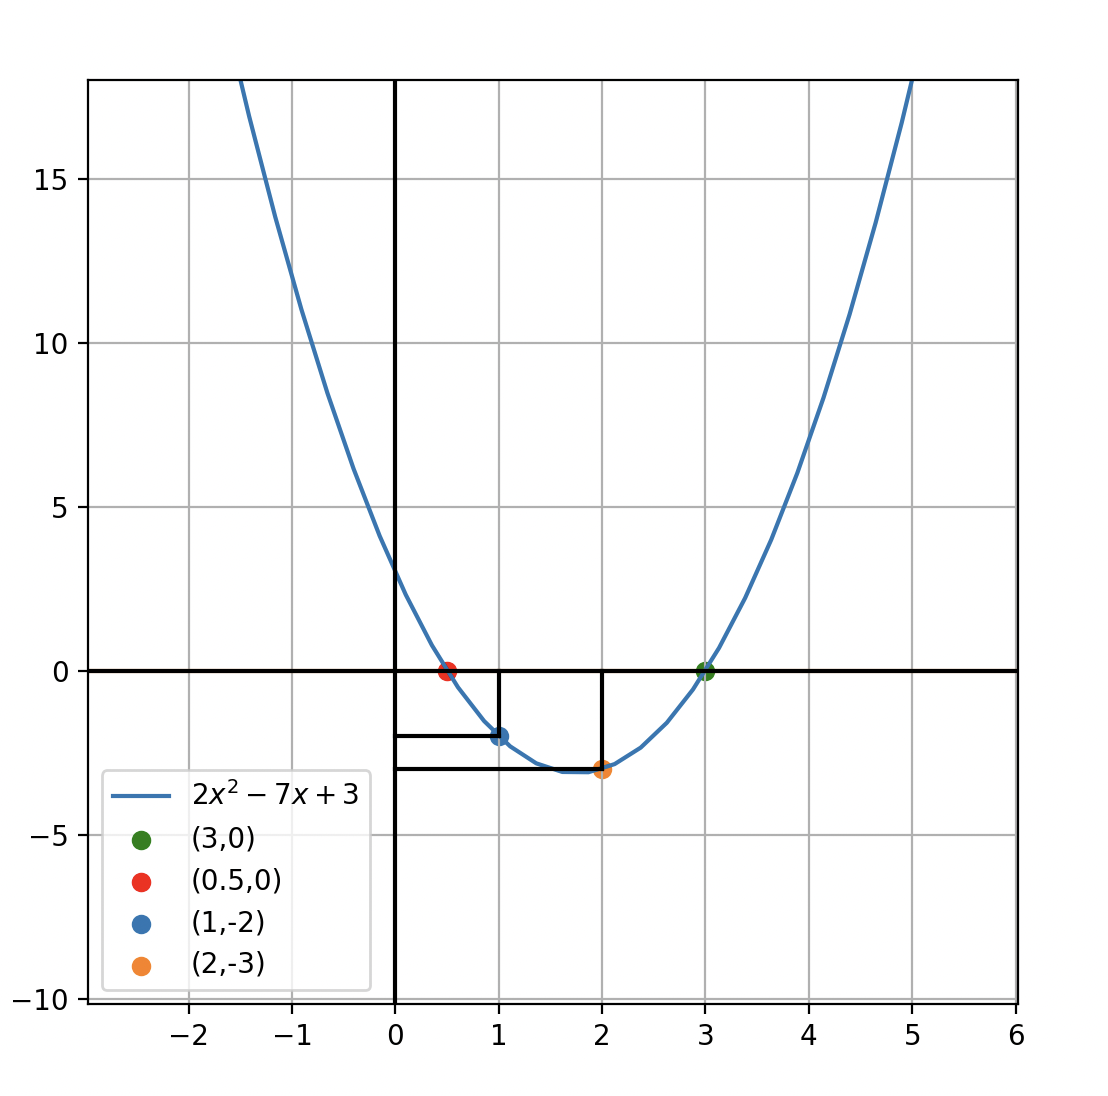
\includegraphics[width=0.9\columnwidth]{Figs/9416.png}
    \caption{Plot}
    \label{fig:placeholder}
\end{figure}


\end{document}